\section{Packet Filtering}%
\label{sec:packet_filtering}

\subsection{Funktionsweise}%

Netzwerkpakete werden je nach bestimmten Parametern akzeptiert oder zurückgewiesen,
z.\,B.:
\begin{itemize}
  \item Quelladresse, Quellport (falls das Protokoll das Konzept kennt)
  \item Zieladresse, Zielport (falls das Protokoll das Konzept kennt)
  \item Flags
\end{itemize}

Beispiel: TCP/IP
\begin{center}
  \begin{tabular}{cccccccc}
    \toprule
    \textbf{Layer} & \multicolumn{7}{c}{\textbf{Protokoll}}\\
    \midrule
    5-7 & Telnet & TFTP & FTP & SMTP & SNMP & DNS & \dots\\
    \midrule
    4 & \multicolumn{3}{c}{TCP} & \multicolumn{3}{c}{UDP}\\
    \midrule
    3 & IP & RARP & ARP & ICMP\\
    \midrule
    2 & \multicolumn{7}{c}{Logical Link Control \& Media Access Control}\\
    \midrule
    1 & \multicolumn{7}{c}{IEEE 802.2, Ethernet, ISDN, \dots}\\
    \bottomrule
  \end{tabular}
\end{center}

\begin{figure}[h]
  \centering
  \begin{subfigure}[c]{0.45\textwidth}
    \centering
    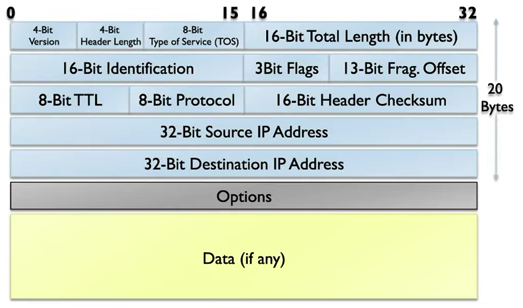
\includegraphics[width=1.0\textwidth]{bilder/ipv4_header.png}
    \subcaption{IPv4 Header}
    \label{fig:ipv4_header}
  \end{subfigure}
  \begin{subfigure}[c]{0.45\textwidth}
    \centering
    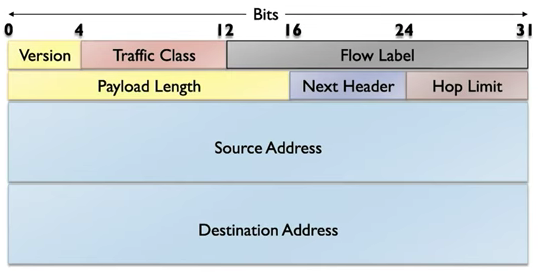
\includegraphics[width=1.0\textwidth]{bilder/ipv6_header.png}
    \subcaption{IPv6 Header}
    \label{fig:ipv6_header}
  \end{subfigure}

  \begin{subfigure}[c]{0.45\textwidth}
    \centering
    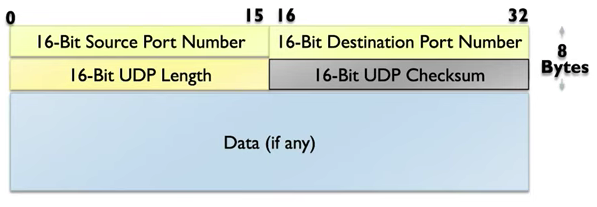
\includegraphics[width=1.0\linewidth]{bilder/udp_header.png}
    \subcaption{UDP Header}
    \label{fig:udp_header}
  \end{subfigure}
  \begin{subfigure}[c]{0.45\textwidth}
    \centering
    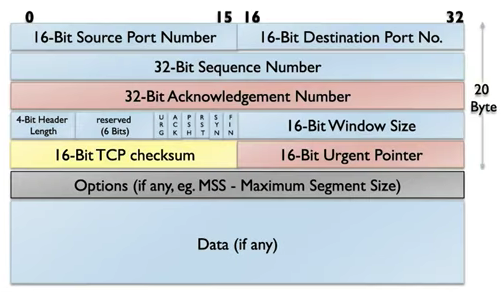
\includegraphics[width=1.0\linewidth]{bilder/tcp_header.png}
    \subcaption{TCP Header}
    \label{fig:tcp_header}
  \end{subfigure}
  \caption{Header von verschiedenen Protokollen}
\end{figure}

\paragraph{Regeln von Packet Filtern}%
\label{par:regeln_von_packet_filtern}

Die Regeln anhand von Flags, Adressen und Ports erstellt werden.
Man kann auch Pakete nach Inhalten filtern.

\paragraph{Arten von Regeln}%
\label{par:arten_von_regeln}

Erlaubende Regeln:
\begin{itemize}
  \item explizit bestimmten Zugang erlauben
  \item anderer Traffic wird normalerweise abgelehnt
\end{itemize}

Verbietende Regeln:
\begin{itemize}
  \item explizit bestimmte Pakete ablehnen
  \item anderer Traffic wird normalerweise zugelassen
\end{itemize}

Die Reihenfolge der Regeln ist wichtig.
Große Anzahl an Regeln ist meist verwirrend.
Best practice kann sein: verbiete alles außer anderweitig angegeben.
Beispiel:
\begin{itemize}
  \item \texttt{deny ip host 205.205.205.1 any}

    verbietet alle IP Pakete vom angegebenen Host

  \item \texttt{permit tcp host 205.205.205.1 any}

    erlaubt alle TCP Pakete vom angegebenen Host
\end{itemize}

Ingress filtering (Eingangskontrolle): filtert eingehende Pakete.
Verbietet Zugang von verdächtigen Quelladressen.

Egress filtering (Ausgangskontrolle): filtert ausgehenden Traffic.
Es dürfen nur Pakete das Netzwerk verlassen, deren Quelladresse im Netzwerk ist.
Falls Traffic von einem Knoten abgelehnt wird, dann ist das ein guter Kandidat für ein
Auditing.

Protokolle filtern: Dienste haben bestimmte Protokolle.
Daumenregel: erlaube nur Dienste, die wirklich benötigt werden.
Beispiele:
\begin{itemize}
  \item ICMP wird vollständig gefiltert
  \item UDP wird vollständig gefiltert
  \item TCP wird nur auf Port 80 erlaubt
  \item bei ICMP wird nur echo erlaubt
\end{itemize}

\paragraph{Probleme}%

Gefahr des Spoofings: externe Hosts können eine falsche Quelladresse vortäuschen und
weitere Authentifizierung ist nötig.
VPN wäre eine Lösung.

Routing: Pakete können Informationen zur Rückroute enthalten.
Die Routingtabelle könnte überschrieben werde.
Heutzutage aber kein Problem mehr.

Fragmentierung: Header eines Paketes könnte geteilt werden, sodass die Firewall nicht auf
den Header zugreifen kann.
Heutzutage auch kein Problem mehr.

Löcher: Chef möchte Sonderregelung, Angreifer nutzt das aus.

\subsection{Dynamisches Packet Filtering}%
\label{sub:dynamisches_packet_filtering}

Filterregel wird on-the-fly erstellt und gelöscht, nachdem die Verbindung geschlossen
wurde.
Der Filter beobachtet den ausgehenden Traffic und erstellt reflexive Regeln, aber nur
solange sie benötigt werden.
Beispiel: wenn eine ausgehende Verbindung zu 217.0.12.12:23 aufgebaut wird, dann wird eine
Regel erstellt, die eingehenden Traffic von 217.0.12.12:23 erlaubt.

\paragraph{Probleme}%

Regeln sind angreifbar indem falsche RST (reset) Pakete gesendet werden.
Ausgehender Traffic wird nicht gefiltert (Trojaner, Viren).
